%%  Assignment 1, MATH5425 Graph Theory, 2012


\documentclass[12pt,a4paper]{article}

\usepackage{amsmath,amssymb,latexsym}
\usepackage{graphicx, multirow, polynom}



\addtolength{\topmargin}{-3\baselineskip}
\addtolength{\textheight}{6\baselineskip}
\addtolength{\textwidth}{2cm}
\addtolength{\oddsidemargin}{-1cm}
\addtolength{\evensidemargin}{-1cm}

\def\nfrac#1#2{{\textstyle\frac{#1}{#2}}}

\newcommand{\nc}{\newcommand}
\def \qedbox{\hfill\vbox{\hrule\hbox{\vrule
height1.3ex\hskip0.8ex\vrule}\hrule}}

\pagestyle{plain}

\setlength{\parskip}{\baselineskip}
\setlength{\parindent}{0mm}


\begin{document}

\vspace*{-\baselineskip}

\begin{center}
{\large {\bf  SCHOOL OF MATHEMATICS AND STATISTICS\\  
            UNIVERSITY OF NEW SOUTH WALES}}
\end{center}

\vspace*{-\baselineskip}

\begin{center}
{\large {\bf Extension 2 Tips and Tricks \qquad Open Day 2012 }}
\end{center}

\vspace*{-\baselineskip}

\begin{center}
{\bf  { \copyright UNSW MATHSOC 2012.}}
\end{center}

This handout was written by Peter Ayre, Johann Blanco, Varun Nayyar, Colin Zhang, Daniel Le and Georgia Tsambos. The suggestions made are those of the authors, and are not officially endorsed by the School of Mathematics and Statistics or the Faculty of Science.

Please be ethical with this resource. It is for the use of Open Day attendees and their friends, so {\bf please do not repost it on other forums or groups without asking for permission}. If you choose to come to UNSW (which we hope you do!), please consider supporting us by joining our society!  Happy studying and good luck :)

Many thanks to the School of Mathematics and Statistics and the Faculty of Science for helping us out with this event, and for being awesome in general!

if you spot any errors, please email them to g.tsambos@student.unsw.edu.au.\\[2mm]

{\bf {\large Contents:}
\begin{enumerate}
\item[1. ] l'Hopital's rule
\item[2. ] Advanced Combinatorics
\item[3. ] Quick Integration by Substitution
\item[4. ] Heaviside Method
\item[5. ] General Exam Tips
\item[6. ] Calculator tricks
\end{enumerate}}


%L'Hopital's rule
\newpage
\noindent {\bf \Large 1. L'Hopital's rule}\quad
\bigskip 
\\[2mm]
L'Hopital's Rule is a method of evaluating limits involving indeterminate forms. The rule is named after 17th century French mathematician Guillaume de l'Hopital and was published in 1696.\\[2mm]
In it's simplest form, l'Hopital's rule states that if
\[
\lim_{x\rightarrow c} f(x) = \lim_{x\rightarrow c} g(x) = 0 \text{ or } \pm \infty ,
\]
then
\[
\lim_{x\rightarrow c} \frac{f(x)}{g(x)} = \lim_{x\rightarrow c} \frac{f'(x)}{g'(x)}.
\]

Moreover, l'Hopital's rule may be applied iteratively. Continuing the previous example, if
\[
\lim_{x\rightarrow c} f'(x) = \lim_{x\rightarrow c} g'(x) = 0 \text{ or } \pm \infty ,
\]
then
\[
\lim_{x\rightarrow c} \frac{f(x)}{g(x)} = \lim_{x\rightarrow c} \frac{f'(x)}{g'(x)} = \lim_{x\rightarrow c} \frac{f''(x)}{g''(x)}.
\]

\begin{itemize}
\item[{\bf Eg. 1:}] Evaluate $\displaystyle{ \lim_{x\rightarrow 1} \frac{ 2\log_e x }{x-1}}$.\\[2mm]

{\bf Solution:} Setting $f(x) = 2 \log_e x, g(x) = x-1$, we note that 
\[
\lim_{x\rightarrow c} f(x) = \lim_{x\rightarrow c} g(x) = 0.
\]
Then by l'Hopital's rule,
\[
\lim_{x\rightarrow 1} \frac{2 \log_e x}{x-1} = \lim_{x\rightarrow 1} \frac{ \frac{d}{dx} (2 \log_e x)}{ \frac{d}{dx} (x-1)} = \lim_{x\rightarrow 1} \frac{\frac{2}{x}}{1} = 2. \thickspace \Box
\]
\end{itemize}


\bigskip

\noindent{\bf Useful note:}
Identities such as 
\[
\lim_{k\rightarrow 0} \frac{\sin x}{x}, \lim_{k\rightarrow 0} \frac{\tan x}{x} 
\]
may be computed quickly by l'Hopital's rule (meaning you need to remember less!)
\begin{align*}
\lim_{k\rightarrow 0} \frac{\sin x}{x} &= \lim_{k\rightarrow 0} \frac{\cos x}{1} = 1\\[2mm]
\lim_{k\rightarrow 0} \frac{\tan x}{x} &= \lim_{k\rightarrow 0} \frac{\sec ^2 x}{1} = 1
\end{align*}
 Only differentiate again if the limit is again indeterminate $(\frac{0}{0}, \frac{\infty}{\infty}, \frac{-\infty}{-\infty})$. \\[2mm]
 
 {\bf Disclaimer! } l'Hopital's rule only initially appears in university level calculus and is not an "approved method" of the Board of Studies. As such, in examinations please use HSC methods for working and utilise l'Hopital's rule {\it only} for checking work and remembering identities.
 
 \begin{itemize}
 \item[{\bf Eg. 2}] Evaluate $\displaystyle{ \lim_{x\rightarrow 2} \frac{ x^3 - 2x^2 + 5x - 10 }{ x-2 } }$.
 \bigskip
 
 {\bf Solution: HSC method}
 \begin{enumerate}
 \item[Step 1. ] Factorise $p(x) = x^3 - 2x^2 + 5x - 10$. Observe that p(2)=0, then \\[2mm]
\polylongdiv{x^3-2x^2+5x-10}{x-2}\\[2mm]
So $p(x)= (x-2)(x^2 + 5)$.
\item[Step 2. ] Thus,
\begin{align*}
\lim_{x\rightarrow 2} \frac{ x^3 - 2x^2 + 5x - 10 }{ x-2 } &= \lim_{x\rightarrow 2} \frac{ (x-2)(x^2 + 5)}{ x-2 } \\[2mm]
&=  \lim_{x\rightarrow 2} x^2 + 5 = 9. \thickspace \Box
\end{align*}
 \end{enumerate}
 
\bigskip
\bigskip 
 {\bf Alternative solution: l'Hopital's rule}\\[2mm]
 Note that 
 \[
 \lim_{x\rightarrow 2}{ x^3 - 2x^2 + 5x - 10 } =  \lim_{x\rightarrow 2} x -2 = 0.
 \]
 Then by L'Hopital's rule,
 \begin{align*}
 \lim_{x\rightarrow 2} \frac{ x^3 - 2x^2 + 5x - 10 }{ x-2 } &= \lim_{x\rightarrow 2} \frac{ \frac{d}{dx} ( x^3 - 2x^2 + 5x - 10 )}{\frac{d}{dx} (x-2) }\\[2mm]
 &=  \lim_{x\rightarrow 2} \frac{ 3x^2 -4x +5 }{ 1 }\\[2mm]
 &= 3(2)^2 - 4(2) + 5= 9. \thickspace \Box
 \end{align*}
 
 \end{itemize}


% Enumeration and probability
\newpage
\noindent {\bf \Large 2. Advanced Combinatorics }\quad 
\bigskip

Counting, also called  'enumeration' or 'combinatorics', can be one of the most demanding and difficult portions of an HSC exam. Probability, a related area, can also be quite challenging.

\bigskip

\noindent {\bf General tips: }
\begin{itemize}
\item For these problems, {\it always} set out your working clearly. In most questions, this means listing the choices to be made and the number of options in each case; and then combining these by addition or multiplication to get the final answer.
\item Remember to count everything! Don't count anything twice! These are obvious but they are not always easy to put into practice.
\item It is useful to spend some time determining what type of problem it is. Does it involve arrangements? Are they ordered? If it's probability, is it binomial? Asking these questions can make it much easier to see the 'best' way to do the question.
\end{itemize}

{\bf What type of question is this?}

Counting problems (�enumeration�) in the HSC can be split into three broad categories: ordered selections (permutations), unordered selections (combinations) and ordered arrangements. There have been instances where counting problems were solved as probability ones and vice versa. Make sure you know what type of question you're solving!

\begin{enumerate}
\item[{\bf Eg. 1: }] (MX1 1995, Q3a)\\
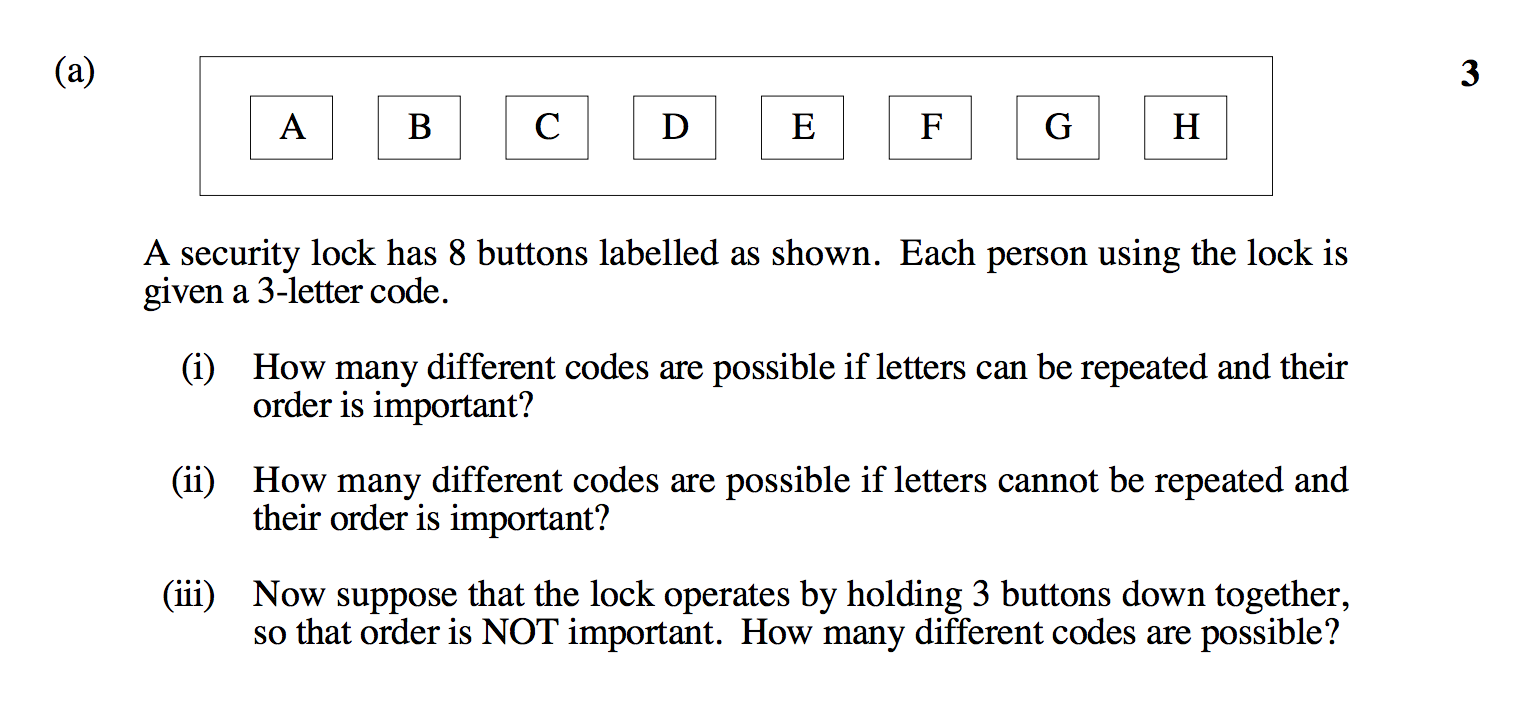
\includegraphics[scale = 0.5]{mx1_1995_3a.png}
{\it Problem type:}\\[2mm]
Parts (i) and (ii) are {\bf permutation} problems. \\
Part (iii) is a {\bf combination} problem. 
\bigskip
\bigskip

\item[{\bf Eg. 2: }] How many ways can the letters of the word INSURABLE be arranged in a row?\\[2mm] 
{\it Problem type:}\\[2mm]
This is a {\bf ordered arrangement} question. Order is relevant, and repetitions are not allowed.\\[2mm] 
\bigskip

\item[{\bf Eg. 3: }]  (MX2 1996 (4c) part i:)\\[2mm]
Consider a lotto style game with a barrel containing twenty similar
balls labelled 1 to 20. In each game, four balls are drawn, without replacement, from the 
twenty balls in the barrel. The probability that any particular number is drawn in the game is 0.2. Find the 
probability that the number 20 is drawn in exactly two of the next five games played. \\[2mm]
{\it Problem type: }\\[2mm]
This is a {\bf binomial probability} question. 
What are the values of n? p? q? r?\\[2mm] 
\bigskip

\item[{\bf Eg. 4: }] A group of 12 people are to be divided into discussion groups. In how many ways can the discussion groups be formed if there are 3 groups containing 4 people each? \\[2mm]
{\bf Your working:}
\bigskip
\bigskip
\bigskip
\bigskip
\bigskip
\bigskip
\bigskip
\bigskip
\bigskip
\bigskip
\bigskip

{\bf Solution: }
\begin{enumerate}
\item[ 1. ] Select four people from the twelve to go into the first group. There are ${{12}\choose{4}}$ ways of doing this.\\
\item[ 2. ] Select four people from the remaining eight to go into the second group. There are ${{8}\choose{4}}$ ways of doing this.\\
\item[3. ] Select four people from the remaining four to make the last group. There are ${{4}\choose{4}}$ ways of doing this.\\
\item[4. ] These groups are not different from each other, so we must divide by 3! to avoid counting some ways more than once. \\ 
\end{enumerate}

{\it Answer: } $\displaystyle{ \frac{ { {12}\choose{4}} {{8}\choose{4}} {{4}\choose{4}} }{3!} }.$ $\Box$

\end{enumerate}

\bigskip
\bigskip

Now the HSC method looks easy, just writing down the answer. However, for the harder problems you may encounter, it helps to write down your logic. This way, silly mistakes are easier to spot as the working is clear and concise.

Let's try a harder example:

\begin{enumerate}
\item[{\bf Eg. 5: }] (MX1 2000 (6):)\\[2mm]
 A standard pack of 52 cards consists of 13 cards of each of the four suits: spades, hearts, clubs and diamonds.
 \begin{itemize}
 \item[(a)]  In how many ways can six cards be selected without replacement so that exactly two are spades and four are clubs?  
 \item[(b)] In how many ways can six cards be selected without replacement if at least five cards must be of the same suit?\\[2mm]
 \end{itemize}

{\bf Solution: }
\begin{itemize}
\item[(a)]
\begin{enumerate}
\item[1. ] Select two spades for the six card hand. There are ${{13}\choose{2}}$ ways to do this.
\item[2. ] Select four clubs. There are  ${{13}\choose{4}}$ ways to do this.\\[2mm]
\end{enumerate}
{\it Answer: } ${{13}\choose{2}}{{13}\choose{4}}$.\\[2mm]
\item[(b)] We consider two cases: \\[2mm]
{\it Case 1: 5 of one suit} 
\begin{enumerate}
\item[1. ] Select the suit which five cards appear from. There are 4 ways of doing this.
\item[2. ] Select 5 cards from this suit. There are ${{13}\choose{5}}$ ways to do this.
\item[3. ] Select the last card from the remaining 39 cards of the suit not picked. There are ${{39}\choose{1}}$ ways to do this.
\end{enumerate}
{\it Subtotal: } $4 \times {{13}\choose{5}} \times {{39}\choose{1}}$. \\[2mm]

{\it Case 2: 6 of one suit}
\begin{enumerate}
\item[ 1.] Select the suit which appears in the hand. There are 4 ways of doing this.
\item[2. ] Select six cards from one suit. There are  ${{13}\choose{6}}$ ways to do this.
\end{enumerate}
{\it Subtotal: } $4\times {{13}\choose{6}}$.\\[2mm]
{\it Answer: }   $4 \times {{13}\choose{5}} \times {{39}\choose{1}} + 4\times {{13}\choose{6}}. \medspace \Box$

\end{itemize}
\end{enumerate}
\bigskip
Try these yourself, using the new method:

\begin{enumerate}
\item[{\bf 1. }]  ( MX1 2001 (2c) part ii)\\
 How many arrangements of the letters of the word ALGEBRAIC are possible if the vowels must occupy the 2nd, 3rd, 5th and 8th positions?

\item[{\bf 2. }] ( MX2 2002 (4c) part ii)\\
From a pack of nine cards numbered 1, 2, 3, $\ldots$ , 9, three cards are drawn at random and placed from left to right. What is the probability that the digits are drawn in descending order? [Hint: for example, 9, 5 and 1 � in that order]

\item[{\bf 3. }] ( MX2 2003 (4c) part i)\\
 A hall has n doors. Suppose that n people choose any door at random to enter the hall. In how many ways can this be done?
\end{enumerate}

{\bf Finding the best way}

Rushing into a question can cause silly mistakes, but this may mean you also fail to recognise a better way to do the question. When given what appears to be a non-standard question, it is worth your while to consider how best to approach the question.

\begin{itemize}
\item[{\bf Eg. 6: }] (MX2 1996 (4c) part iv)\\
 Let $j$ be an integer from 4 to 20. Show that the probability that, in any one game, j is the largest of the four numbers drawn is 
\[ \displaystyle{ \frac{ {{j-1}\choose{3}} }{ {{20}\choose{4} }} }\]
\bigskip.

{\bf Solution: }
The answer is actually simple � but requires a knowledge of what is going on in the lotto game, and thus probability and enumeration in general.\\[3mm]
What is the total number of possibilities in this lotto game? ${{20}\choose{4}}$.\\[3mm]
We now have to find the number of favourable outcomes. So given an arbitrary integer j from 4 to 20 � how many favourable outcomes are there? That is, how many times will the other three balls picked have a value less than j?\\[3mm]
Let us re-state the question as: �Given an integer $j$ from 4 to 20, how many ways can we pick three more numbers that all have a value less than j?� . We have $j-1$ numbers to pick from, and we select three of them. Simple.\\[3mm]
Not convinced? Let us set $j = 4$. So now we want to find out how many times the next three balls drawn will be less than 4. There is only one solution: 1, 2 and 3 � it doesn�t matter what order they�re picked in. �Mathematically�, there is ${{3}\choose{3}} = 1$ way of doing this selection. $\medspace \Box$

\end{itemize}

Here is another question where you may be tempted to overcomplicate things:
\begin{itemize}
\item[{\bf Eg. 7: }] One semester, 65\% of the students studying MATH1231/41 attended all their tutorials, and of these students, 45\% were awarded credit or higher in the final exam. In contrast, only 30\% of the students who did not attend all their tutorials were awarded a credit or higher in the final exam. What percentage of the students studying MATH1231/41 were not awarded credit or higher in the final exam? Of the students awarded a credit or higher in the final exam, what percentage, correct to one decimal place, attended all their tutorials?

\bigskip
{\bf Solution: }\\[2mm]
 You may be tempted to do some weird complex probability binomial thingamajig. But use a tree diagram. Seriously. There are instances in the HSC where in the marker's comments, they say that the most successful responses just used a tree diagram. $\Box$
\end{itemize}

Here's another interesting question:

\begin{itemize}
\item[{\bf Eg. 8: }] (MX2 2004 (5b) part ii)\\
  In how many ways can five students be placed in three distinct rooms so that no room is empty?\\[2mm]
{\bf Solution: }\\[2mm]
This uses a special method called 'dots, lines and dividers'.\\[4mm]
We have five �objects� (students) which we want to place in three rooms. We can visualise a solution in a table like this, where $\bullet$ denotes a person:\\[4mm]

\hspace{40mm}
\begin{tabular}{ c | c | c }
  Room 1 & Room 2 & Room 3 \\
  $\bullet \bullet$   & $\bullet\bullet$ & $\bullet$\\
  $\bullet\bullet\bullet$ & $\bullet$ & $\bullet$ \\
\end{tabular} \\[2mm]

The first solution gives two people in rooms 1 and 2, and one in room 3. Second solution gives three in room 1, and one each in rooms 2 and 3. We can picture these solutions as a row of dots and lines. For example, the first solution above could be represented as $ \bullet \bullet \medspace|\medspace \bullet \bullet \medspace | \medspace \bullet \medspace$.\\[2mm]

So, we have 7 objects - 5 dots and 2 lines - which we must arrange in a row to represent a 'solution'.  \\

Let us pick the places for the 5 dots first. There are C(7, 5) ways of doing this. The remaining 2 lines can be put into the remaining 2 places one way. (Check that you get the same answer when you first choose the places for the lines.)\\

Clearly then here, the answer is ${{7}\choose{5}}$. But this is WRONG! Why?\\

Because this is also a solution: $\bullet \bullet\bullet\bullet| \bullet|$. We require each room to have at least one person. Or, make sure each line has a dot either side of it. How can we do this using the dots and lines method? We set aside 3 dots. We have two dots and two lines remaining and we arrange these as before.\\

\begin{enumerate}
\item[1. ] Arrange the two dots and two lines as before, choosing places for the dots. There are ${{4}\choose{2}}$ ways of doing this.
\item[2. ] Place 1 reserved dot in the first group. There is 1 way of doing this. 
\item[3. ] Place 1 reserved dot in the second group. There is 1 way of doing this.
\item[4. ] Place 1 reserved dot in the third group. There is 1 way of doing this. \\[2mm]
\end{enumerate}
This guarantees that each room will have at least one student in it.\\[2mm] {\it Answer:} \hspace{10mm} ${{4}\choose{2}} \medspace $ :)

\end{itemize}

%Integration by inspection
\newpage
\noindent{\bf \Large 3. Quick Integration by Substitution }\quad
\bigskip

Time is of the essence in the HSC exam and you would like to have as much time as possible to tackle the harder questions at the back end of the paper. While writing good old u-substitutions when integrating might be good for a class test or textbook work, you would rather spend more time pondering that difficult conics question than writing things like:
\begin{center}
"Let $ u=3x \Rightarrow \frac{du}{dx} = 3 \Rightarrow du= 3x\thickspace dx $"
 \end{center}
 
tl;dr Why do it? It's quicker.\\
 
{\bf Simple examples}\\[2mm]
Integration has the lovely property that if you differentiate your answer (provided it's not an evaluated definite integral, for example) � you get what you had to integrate originally. You can do this to check that you're right.
 
 Let's look over a few examples which can be worked out mentally. The constant is omitted.
 
\begin{enumerate}
 \item[{\bf Eg. 1: }] \hspace{20 mm}$\displaystyle{ \int \cos 6x \thickspace dx = \frac{1}{6} \sin 6x }$\\[2mm]
 \item[{\bf Eg. 2: }] \hspace{20 mm}$\displaystyle{ \int \frac{ \cos x - \sin x }{ \cos x + \sin x } \thickspace dx = \log_e | \cos x + \sin x |} $
 \end{enumerate}


If you mull over the above examples, you can see it is not that difficult to determine the mental steps involved in such a calculation. In more difficult examples, the best thing we can do is anticipate what the answer will be � and then "fudge it" until we get what we want.\\[2mm]

{\bf Integration by Inspection}\\[2mm]
For suitable integrals (we will soon see integrals which cannot be solved using this method), we can summarise the method into three steps:
\begin{enumerate}
\item[ 1. ] Anticipate what the integral will be. Guess what sort of primitive function the integral might have.
\item[ 2. ] Differentiate this �guess�, and compare it to what you had originally.
\item[ 3. ] Fudge the �guess� by multiplying/dividing your guess by a constant until you get what you want. 
\end{enumerate}

Let us look at a few examples, keeping in mind that these steps should mostly be done mentally (you may want to do a bit of scribbling in the margin, but the main point is to not require formal substitution):
\begin{enumerate}
\item[{\bf Eg. 3: }]\hspace{20 mm} $\displaystyle{ \int \cos \frac{x}{2} \thickspace dx }$\\[2mm]

{\bf Solution: }
\begin{enumerate}
\item[ 1. ] This uses $\cos$ so our guess will have $\sin$ in it. So let us guess $\sin \frac{x}{2}$, for example.\\[2mm]
\item[ 2. ] We note that $\displaystyle{ \frac{d}{dx} ( \sin \frac{x}{2} ) = \frac{1}{2} \cos \frac{x}{2} }$.\\[2mm]
\item[ 3. ] We have this $\frac{1}{2}$ out the front when we do not want it. So we get rid of it by "fudging".  Let us multiply our guess by 2. Now: $\displaystyle{ \frac{d}{dx} 2 \sin \frac{x}{2} = 2 \frac{1}{2} \cos \frac{x}{2} = \cos \frac{x}{2} }$. So $\displaystyle{ \int \cos \frac{x}{2} \thickspace dx\text \medspace =\medspace 2 \sin \frac{x}{2}}$, which is what we want! $\Box$\\
\end{enumerate}


\bigskip
\bigskip
\item[{\bf Eg. 4: }] \hspace{20 mm}$\displaystyle{ \int \frac{x}{x^2 +5} \thickspace dx}$\\[2mm]

{\bf Solution:}
\begin{enumerate}
\item[1. ] The numerator is in the form of a derivative of the denominator. So we will "guess" that this integral is a log. Let's guess $\log_e(x^2+5)$.\\[2mm]
\item[2. ] We note that $\displaystyle{ \frac{d}{dx} \log_e(x^2+5) = \frac{2x}{x^2+5} }$.\\[2mm]
\item[3. ]  We have this 2 out the front when we don't want it. So we get rid of it by �fudging� - let's divide our guess by 2. Now
\[
\frac{d}{dx}\thickspace  \frac{1}{2} \log_e (x^2 + 5) = \frac{1}{2} \times \frac{2x}{x^2 +5} =   \frac{x}{x^2 +5}. \\
\]
So 
\[
\int \frac{x}{x^2 +5} \thickspace dx =  \frac{1}{2} \log_e (x^2 + 5) .
\thickspace \Box
\]
\end{enumerate}

\end{enumerate}
\bigskip
\bigskip

The basic principle is simple. Guess, check and then correct it. Of course it only works if the guess and actual answer differ by a multiplicative constant. For example:

\begin{enumerate}
\item[{\bf Eg. 5:}] \hspace{20 mm}$\displaystyle{\int (x^2+ 1)^2 \thickspace dx}$.\\[4mm]

{\bf Solution: }\\[2mm]
\begin{enumerate}
\item[1. ] This kind of looks like a problem where we integrate $u^2$ for example, so let us 'guess'  $(x^2 + 1)^3$.\\[2mm]
\item[2. ] We differentiate: 
\[
\frac{d}{dx}\thickspace (x^2 + 1)^3 = 6x (x^2 + 1)^2.
\]
\item[3. ] We have $6x$ out the front and don't want it, so 
\[
\int (x^2 + 1)^2 \thickspace dx = \frac{1}{6x} (x^2 +1)^3.
\]
But $\displaystyle{ (x^2 + 1)^2 \thickspace dx = \frac{x^5}{5} + \frac{2x^3}{3} + x}. \thickspace \Box$ 
\end{enumerate}

\end{enumerate}

We note here that $6x$ is not a multiplicative constant, so it doesn't work. Why? Best explanation is that we can consider $x$ to be a variable. It is not a constant. \\[2mm]
Lastly, let's try a difficult one:\\[2mm]

\begin{enumerate}
\item[{\bf Eg. 6:}] \hspace{20 mm} $\displaystyle{ \int \frac{1}{\sqrt{ 3x + 4 }}\thickspace dx }$.\\[4mm]
{\bf Solution: }\\
\begin{enumerate}
\item[1. ] Before we guess, we note that if we were to make a substitution, it would be $u= 3x + 4$. Hence when we 'substitute', $du$ and $dx$ differ just by a constant and we can 'guess' a solution. If you're not convinced, replace $x$ with $x^2$ and see that we can't use this method.\\[2mm]
\item[ 2. ] Then 
\[
\frac{d}{dx} \thickspace \sqrt{3x + 4} = \frac{1}{2} (3x + 4)^{-\frac{1}{2}} \times 3 = \frac{3}{2\sqrt{3x + 4}}.
\]\\
\item[3. ] We are out by a factor of $\frac{3}{2}$, so we adjust by dividing our guess by  $\frac{3}{2}$. Our new guess is $\displaystyle{ \frac{2}{3} \sqrt{3x +4 } }$. Now we note that 
\[
\frac{d}{dx} \thickspace (\frac{2}{3} \sqrt{3x+4}) = \frac{2}{3} \times \frac{1}{2} (3x+4)^{-\frac{1}{2}} \times 3 = \frac{1}{\sqrt{ 3x+4 }}.
\]
So $\displaystyle{ \int \frac{1}{\sqrt{ 3x + 4 }}\thickspace dx =   \frac{2}{3} \sqrt{3x +4 }}$. $\Box$
\end{enumerate}
\end{enumerate}

{\bf Summary}\\[2mm]
Integration by inspection certainly saves time. However, it does not replace the substitution method! 
If we look at the example above, that is quite difficult work. Your aim in this should not be to be able to do all the steps in your head. In fact, skipping steps and doing things mentally can cause mistakes. However as this has an easy 'check', you can still save time by doing these integrations by inspection.\\[2mm]
The aim of this is to make you not waste valuable time writing out the substitution formally. By using inspection/inspiration to see what the integral could be, you can solve it much faster.\\[2mm]
Try these yourself:
\begin{enumerate} 
\item[1. ] $\displaystyle{ \int\frac{ \sin \sqrt{u} }{\sqrt{u}} \thickspace du }$
\item[2. ] $\displaystyle{ \int \sin^4 x \cos x \thickspace dx }$
\item[3. ] $\displaystyle{ \int x^5 \sqrt{ x^6-2 } \thickspace dx}$
\item[4. ] $\displaystyle{ \int e^{-x} \sec^2 (e^{-x}) \thickspace dx }$
\item[5. ] $\displaystyle{ \int  (2x+5)^9\thickspace dx }$
\item[6. ] $\displaystyle{ \int  y e^{y^2} \thickspace dy}$
\item[7. ] $\displaystyle{ \int e^{x^{-1}} x^{-2} \thickspace dx}$
\item[8. ] $\displaystyle{ \int \frac{ 2e^x }{ 3+ e^{2x} }\thickspace dx }$
\item[9. ] $\displaystyle{ -\int \frac{ \sin^5{x^{-1}} \cos\frac{1}{x}}{x^2} \thickspace dx }$
\end{enumerate}



%Heaviside method
\newpage
\noindent{\bf \Large 4. Heaviside method }\quad
\bigskip

A rational function is a function of the form $\dfrac{p(x)}{q(x)}$ where $p$ and $q$ are polynomials.
\begin{itemize}
\item[{\bf Eg. 1:}] \hspace{20mm}$\dfrac{3x + 3}{2x^{2} + x + 5}$ \\
\end{itemize}
When evaluating the integral of a rational function, it is sometimes necessary to 'decompose' it into a linear combination of linear factors of the denominator in order to directly compute the integral.

We can do this by a method which you have learnt in school, called the {\it partial fraction decomposition}. \\
\begin{itemize}
\item[{\bf Eg. 2:}] \hspace{20mm} $\displaystyle{ \int\limits_{}^{} \dfrac{dx}{(x-2)(x+1)(3-x)} }$
\end{itemize}

The integrand can be written as $\dfrac{A}{x-2} + \dfrac{B}{x+1} + \dfrac{C}{3-x}$ where A, B and C are constants. The following method is what you may have learnt in school to solve for the constants A, B and C. \\

\begin{enumerate}
\item[1. ]$\dfrac{dx}{(x-2)(x+1)(3-x)} = \dfrac{A}{x-2} + \dfrac{B}{x+1} + \dfrac{C}{3-x}$\\[2mm]
\item[2. ] Multiply both sides by the denominator of the LHS to get
\[
1 = A(x+1)(3-x) + B(x-2)(3-x) + C(x-2)(x+1) \\[2mm]
\]
\item[3. ] To solve for $A$, we eliminate $B$ and $C$ from our equation. Set $x = 2$:
\[
1 = A(3)(1) \Rightarrow A = \dfrac{1}{3}\\[2mm]
\]
\item[4. ] To solve for $B$, we can eliminate $C$ by setting x = -1:
\[
1 =  B(-3)(4) \Rightarrow B = -\dfrac{1}{12}
\]
\item[5. ] To solve for $C$, we can set x to anything other than 2 or -1 since the equation is true for all values of $x$:
\[
1 = \dfrac{1}{3}(1)(3) - \dfrac{1}{12}(2)(3) + C(2)(1) \Rightarrow C = -\dfrac{1}{4}
\]
Hence $\dfrac{dx}{(x-2)(x+1)(3-x)} = \dfrac{1}{3(x-2)} - \dfrac{1}{12(x+1)} - \dfrac{1}{4(3-x)}. \medspace \Box$

\end{enumerate}
\bigskip
\bigskip

Using the Heaviside cover-up method, you can write down the constants without doing the tedious working out above!

\begin{itemize}
%\item{1. ] $\frac{dx}{(x-2)(x+1)(3-x)} = \frac{A}{x-2} + \frac{B}{x+1} + \frac{C}{3-x}$
\item[1. ] $\displaystyle{ \frac{dx}{(x-2)(x+1)(3-x)} = \frac{A}{x-2} + \frac{B}{x+1} + \frac{C}{3-x}}$.\\[2mm]
\item[2. ] For A, `cover-up' the $(x-2)$ on the LHS and set $x = 2.$
\[
A = \dfrac{1}{(2+1)(3-2)} = \dfrac{1}{3}
\]
\item[3. ] Similarly for B and C, `cover-up' their respective denominators on the LHS and set x to their respective zeros.
\begin{align*}
B &= \dfrac{1}{(-1-2)(3-(-1))} = -\dfrac{1}{12}\\[2mm]
C^{*} &= \dfrac{1}{(3-2)(3+1)} = \dfrac{1}{4}. \medspace \Box
\end{align*}
\end{itemize}

Note we let $C$ equal to the negative of $C^{*}$ since $(3-x) = -(x-3)$.

Here's an easier one for you to try:
\begin{itemize}
\item[{\bf Eg. 3: }] \hspace{20mm} $\dfrac{1}{x(1+x)} = \dfrac{A}{x} + \dfrac{B}{1+x}$
\end{itemize}
You should get $A = 1, B = -1$.\\[2mm]

\begin{itemize}
\item[{\bf Eg. 4: }] $\dfrac{1}{(x-1)^{2}(x+2)} = \dfrac{A}{(x-1)^{2}} + \dfrac{B}{x-1} + \dfrac{C}{x+2}$
\end{itemize}

{\bf Solution: }
\begin{enumerate}
\item[1. ] For $A$, `cover-up' the $(x-1)$ on the LHS and set x = 1.
\[
A = \dfrac{1}{3}
\]
\item[2. ] For $C$, `cover-up' the $(x+2)$ on the LHS and set x = -2.
\[
C = \dfrac{1}{9}
\]
\item[3. ] $B$ cannot be found by the cover-up method. Since we have found $A$ and $C$, we can find $B$ by substituting in any value of $x$ (other than 1 or -2) since the equation is true for (almost) all values of $x$. Setting $x = 0$ we get:
\[
\dfrac{1}{2} = \dfrac{1/3}{1} + \dfrac{B}{-1} + \dfrac{1/9}{2} \Rightarrow B = -\dfrac{1}{9}. \thickspace \Box
\].
\end{enumerate}


Make sure you know when it is appropriate to use partial fraction decomposition when given an integral of a rational function.


%end
% Tips and tricks
\newpage
\noindent {\bf \Large 5. General Exam Tips}\quad 
\bigskip

{\bf Use your reading time well: }\\ Ensure you read everything, even if it takes you longer than the 5 minutes allocated for reading time. This is because you will be thinking about the answers to the harder questions in the back of your head while doing the easy ones. When you get to the those hard questions, you don�t have to stop and think from scratch - you�ve already done some of the thinking earlier on.

{\bf Attempt every question: }\\ Don�t go into an exam with the mentality, �If I can do up to question 7, I�m happy, I�m not going to even look at Question 8�. Consider 2010 HSC, Question 8, part (j) for example - a simple 1 mark question, just taking the limit to infinity of the expression given in (i). Easy 1 markers abound in Question 8, you can usually get at least 2-3 marks without doing any of the actual hard parts of the question.

\begin{itemize}
\item[{(2010, Q8i)}] Use part (e) to deduce that
\[
\frac{\pi^2}{6} - \frac{\pi^3}{8(n+1)} \leq \sum^{n}_{k=1} \frac{1}{k^2} < \frac{\pi^2}{6}.
\]
\item[{(2010, Q8j)}] What is $\displaystyle{ \lim_{n \rightarrow \infty} \sum^{n}_{k=1} \frac{ 1 }{ k^2 }}$?
\end{itemize}


{\bf Getting stuck: }\\ If a question is too hard and the algebra is getting messy (except in Conics), you may have made a mistake - exams are pathologically written to have nice answers pop out (even in Conics).  Check your working carefully and you will almost always find a mixed up sign or missing pro-numeral. \\[2mm]
Also, if you are getting stuck, don�t keep wasting time - this might force you to rush near the end. Just  attempt everything else you can and then come back to the skipped questions - something helpful might occur to you while attempting other questions.\\

{\bf Making notes: }\\ My friend in high school essentially re-wrote the Cambridge textbook into a 112 page behemoth which he claimed to be his notes. He didn�t end up doing all that well, which brings me to notes - the briefer, the better. My notes took up a sum total of 12 pages, and even at uni, my notes for an entire maths course rarely take up more than 10 pages. This is because in maths, you need to focus on understanding, rather than memorization. Have only the essential parts in, consider noting only the not-so-obvious results like $\displaystyle{ \lim_{x\rightarrow 0} \frac{sin x}{x}}$. If you are writing more than 10-15 pages, you might be spending too much time on them. \\[2mm]
And of course, make the notes yourselves - another person's notes are useful to learn from, but less useful for exam prep. The 112 page behemoth was quite popular, but it was always hilarious to see my friends searching for formulas in that huge document. Most of the benefit of notes are in making them, not studying them.\\[2mm]

{\bf The new format: }\\ You no longer have 8 questions worth 15 marks each, you have 10 multiple choice for 10 marks and 6 questions worth 15 each - giving you a grand total of 100 marks. I hope your school trials prepare you adequately, but do keep the format change in mind.\\[2mm]

{\bf Induction conclusion: }\\
While doing induction, the conclusion - i.e. if true for n=1, then true for n=2; if true for n=2, then true for n =3, and hence true for all n - is UNNECESSARY. There are no marks allocated in the HSC, simply writing, �Hence true by induction�, is good enough. However this may not hold for your trials - please confirm this with teachers.


% Calculator
\newpage
\noindent{\bf \Large 6. Calculator tricks}

{\bf 1. Using the 'ans' button}\\[2mm]
This is particularly useful when you do not want to type out a number with a lot of decimals, or if you want to substitute into polynomials quickly. We do this by utilizing the fact that the 'ans' button will always store the previously calculated answer.

So if you wanted to find out $43.51238^2 + 43.51238^3+5 x 43.51238^2$, you can simply type into your calculator 43.51238 , press '=' and then type in $ans ^2 +ans ^3 +5 \times ans$.

Another trick is you can perform with the 'ans' button is the {\bf quick substitution trick}. This is useful in situations where you want to find the various values of a function given different variables.

Say you want to find the value of $x^2+6x-32\text{ for }x=3, x=4 \text{ and } x= 5$. All you have to do is type in $ans^2+6\times ans-32 =$ , and follow this up by typing in 3 and pressing '='. Then you can press the up button and '=' to calculate $3^2+6\times3-32$. Repeat this process by typing in $4\medspace \rightarrow \medspace=  \medspace\rightarrow \medspace \text{ 'up' }  \medspace\rightarrow \medspace = $ to calculate  $4^2+6\times4-32$ and so on. This is quite helpful when you are trying to guess and check the root to a cubic.\\[2mm]

{\bf 2. Complex number simplification - the 'pol' function}

This is a useful feature of the calculator which I personally didn't realize till my 2nd year of university.

Type 'shift' and '+', then type in the x and y values of your complex number $x+iy$ separated by a comma. (The comma can be found by pressing 'shift' and the right bracket button.) After pressing '=', you will get the respective 'r' and $\theta$ values of your complex number.

There is a reverse function, 'rec', next to the 'pol' function. This will allow you to convert a complex number in polar form back into rectangular form.\\[2mm]


{\bf 3. Storing function}

You can store arbitrary values into the different letters of your calculator. After getting a value in your calculator, you can press shift and then 'rcl'/'sto' to save that number into a particular letter on your calculator (A,B,C,D,X,Y,M). This value can later be accessed by pressing $\alpha$ and then the respective letter.

\end{document}
